\documentclass{article}%
\usepackage[T1]{fontenc}%
\usepackage[utf8]{inputenc}%
\usepackage{lmodern}%
\usepackage{textcomp}%
\usepackage{lastpage}%
\usepackage[head=40pt,margin=0.5in,bottom=0.6in]{geometry}%
\usepackage{graphicx}%
%
\title{\textbf{Empleados de la ULA protestaron para exigir mejoras salariales}}%
\author{El Nacional Web}%
\date{22/11/2018}%
%
\begin{document}%
\normalsize%
\maketitle%
\textbf{URL: }%
http://www.el{-}nacional.com/noticias/protestas/empleados{-}ula{-}protestaron{-}para{-}exigir{-}mejoras{-}salariales\_260704\newline%
%
\textbf{Periodico: }%
EN, %
ID: %
260704, %
Seccion: %
Protestas\newline%
%
\textbf{Palabras Claves: }%
Universidades, Mérida, Protestas\newline%
%
\textbf{Derecho: }%
2.3, %
Otros Derechos: %
2.2, %
Sub Derechos: %
2.3.4, 2.2.1\newline%
%
\textbf{EP: }%
SI\newline%
\newline%
%
\textbf{\textit{Los manifestantes bloquearon las vías terrestres frente a la sede adminstrativa de la casa de estudios andina}}%
\newline%
\newline%
%
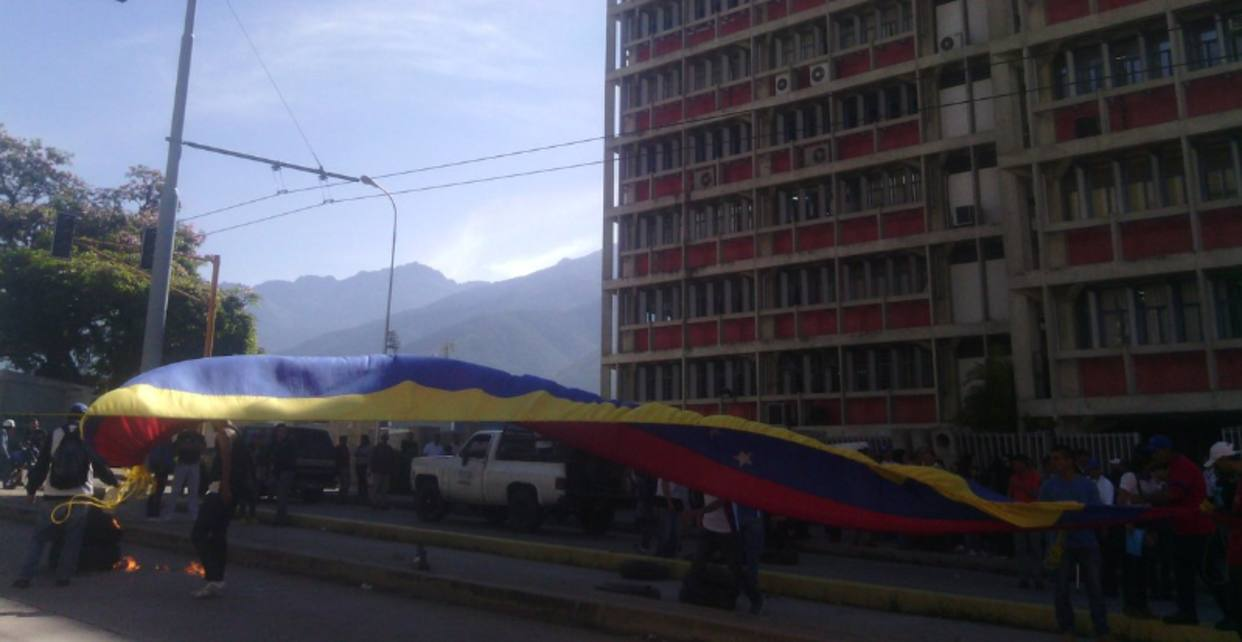
\includegraphics[width=300px]{74.jpg}%
\newline%
%
Empleados de la Universidad de Los Andes (ULA)~protestaron este jueves para exigir el pago de sus salarios~y el cumplimiento de los contratos colectivos de los empleados.%
\newline%
%
Los manifestantes bloquearon las vías terrestres frente al edificio administrativo de la sede de la casa de estudios como señal de protesta.%
\newline%
%
Empleados de diversas instituciones universitarias del país han exigido que se cumpla con las escalas salariales y dotación de insumos para mejorar las universidades.%
\newline%
%
La~Asociación de Empleados de la ULA (Aeula) y el Sindicato de Obreros de la Universidad de Los Andes (Soula) indicaron que las acciones de calles serían más constantes y radicalizadas. Además, publicarán una agenda de protestas de la próxima semana, reseñó Leonardo León.%
\newline%
%
\end{document}